\section{Related work} \label{sec:related}
\subsection{Traditional method}
Originally, total people in the crowd were count by detection. The method in this group mostly using a sliding window with a classifier trained on low-level hand-craft features, such as HOG \cite{dalal2005histograms} and Haar \cite{lin2001estimation}, make attempt to detect all human in the scene. The total count is the number of successful detections.

However, detection approaches become challenging when crowd density increases. Counting by regression was proposed to avoid the hard task of object detection. The approach output one single count number for each input image, without detecting every object. Davies et al \cite{davies1995crowd} trained a linear regression on low-level features such as foreground pixels, edges that output a single count number. Idress et al. \cite{idrees2013multi} combine multiple methods, including SVM with SIFT feature, HOG based head detection, Fourier analysis. Wang et al. \cite{wang2015deep} were the first to use the Convolution neural network (CNN) in crowd counting problems.

While counting by regression avoids difficulty in detection problem, it does not restrain any location information. Lempitsky et al. \cite{lempitsky2010learning} proposed a way to incorporate spatial information into annotated datasets by place a single dot (not bounding-box) at each object of interest and a counting framework to train a regressor that maps input image to density map. Furthermore, the authors argued that dot annotation can be acquired with comparable cost to number-only annotation due to the nature in the way human annotators count a large number of objects. Pham et al. \cite{7410729} improved the method by replacing linear regressors with random forest. Further literature focuses on CNN-based approaches due to the great successes of deep learning and CNN-based approaches in the computer vision paradigm. Early CNN-based approaches in density estimation have been carefully surveyed by Sindagi et al. \cite{SINDAGI20183}.

%%%%%%%%%%%%%%%%%%%%%
\subsection{Recent works}
%ideal: 2 problem 

\subsubsection{Perspective distortion} \hfill

\begin{figure}[htbp]
\centerline{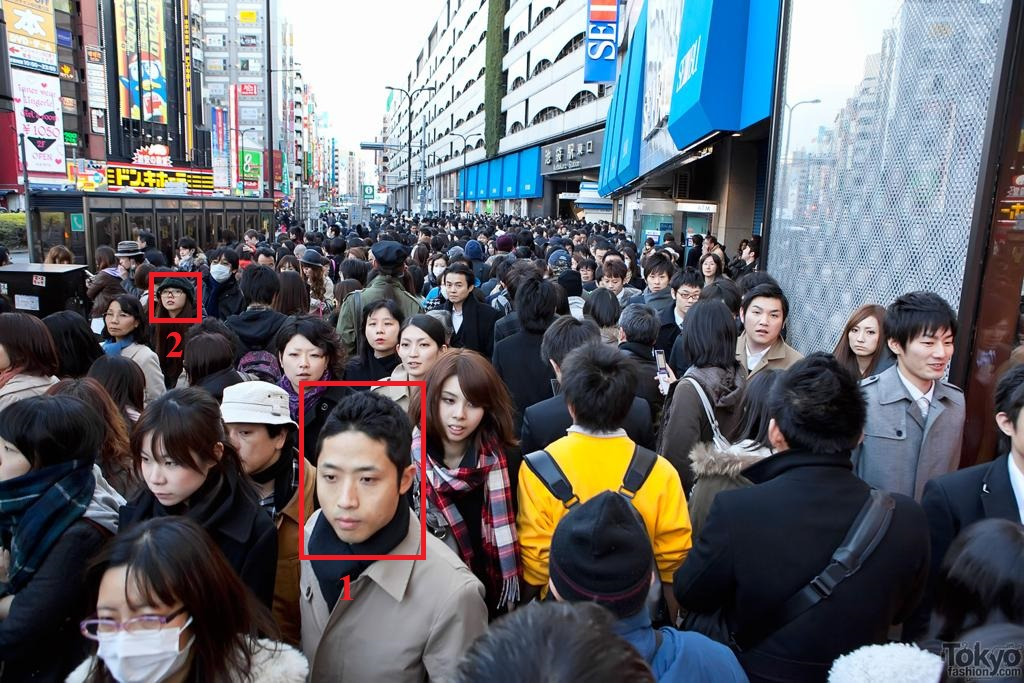
\includegraphics[width=0.4\textwidth]{Picture/problem/part_a_train_IMG_44-annotate-scale.jpg}}
\caption{Scale variation due to perspective distortion. Head in box 1 is bigger than box 2 because people 1 is closer to camera.}
\label{fig:scale}
\end{figure}

Perspective distortion causes people size to variance depending on the camera angle and how far people from the camera is often referred to as a multi-scale problem. The size of people can change between images or vary radically in the same image. The typical CNN model cannot fully adapt to the scale-variance effect. The problem is illustrated in Fig. \ref{fig:scale}. The common solution is a multi-scale feature extraction consists of parallel convolution layers with different receptive field sizes with iconic is multi-column architecture.

Multi-column Convolutional Neural Network (MCNN) \cite{zhang2016single} is among the first model to use multi-columns architecture in crowd counting. MCNN consists of 3 columns, each with different kernel sizes. Feature map output from each column is then concatenated before used to predict the final density map. MCNN was a pioneer to multi-column architecture, in which each column has a different receptive field to copy with a multi-scale problem. Similar works follows \cite{zhang2019crowd, 9053780}. 

However, MCNN fails short when scales vary in the same image. Switch-CNN \cite{sam2017switching} proposed the Switch-classifier, which classifies each image patch to the corresponding CNN column adapts for that specific scale, so does \cite{8965799}. Latter, CAN \cite{liu2019context}, PACNN \cite{shi2019revisiting} merges multi-scale feature with weight-matrix, allowing smoother scale transition across the whole image. 

Another approach is inception-like architecture, inspired from Inception \cite{szegedy2015going}, in which each inception-module, called a multi-scale module, is a mini multi-column convolutional network. The whole network consists of multiple multi-scale modules stack on top of each other, resulting in more scale combinations. SANet \cite{cao2018scale}, MDNet \cite{wang2019multi}, TEDnet \cite{jiang2019crowd}, ADCrowdNet \cite{liu2019adcrowdnet} are notable works. 

\begin{figure}[htbp]
\centerline{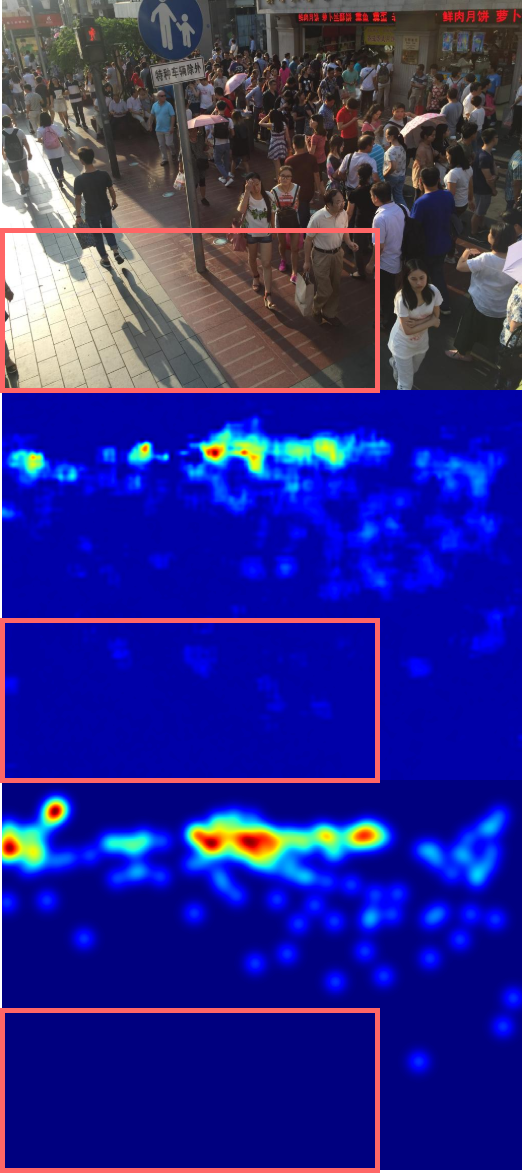
\includegraphics[width=0.4\textwidth]{Picture/problem/background_noise_shb.png}}
\caption{The red box is background and should not contain human.}
\label{fig:noise}
\end{figure}

Background noise is a challenge in which the background
decreases the performing of count counting algorithm.
Background, which is part of an image scene where there are
no people, impacts the result of the predicted people density
map. Empirical experiments show that density result in the
background zone is not always 0 when it should be. Moreover,
background objects, such as tree leaves, have a pattern similar
to a crowd scene, making it easier to have false positives. Sam et
al. \cite{DBLPconfaaaiSamB18} had clearly documented the effect of background noise in
their work. Fig \cite{fig:noise} is an example of C-CNN suffer from background noise

Background noise challenges are tackle, both implicit and explicit approaches. In an explicit approach, authors build a multi-step system, which including a step to remove explicitly remove background from result or input data. Some notable works are: WSRHC \cite{10.1145/3287921.3287980} includes the human-classifier which remove image patches do not contain human; ADCrowdNet \cite{liu2019adcrowdnet} Attention Map Generator segments image into crowd and non-crowd. The implicit approach builds the model so that it is robust to background noise. The common strategies are incorporate contextual information by dilated CNN (CSRNet \cite{li2018csrnet}, CAN \cite{liu2019context}, DMCNN \cite{zhang2019crowd}, \cite{9023874}), combined shallow layers with deep layers (TDF-CNN \cite{DBLPconfaaaiSamB18}, TEDnet \cite{jiang2019crowd}).


